%%%%%%%%%%%%%%%%%%%%%%%%%%%% WEEK 12 %%%%%%%%%%%%%%%%%%%%%%%%%%%%%%%%%%%%
\chapterimage{../Pictures/ttl2.jpg}
\chapter{Parsing Data}

\newcommand{\bb}{white}
\newcommand{\ff}{black}

\newcommand{\sixel}[6]{%
\begin{tikzpicture}[scale=0.333, every node/.style={scale=0.333}]
\matrix[sixelstyle]
{
|[fill=#1]| \& |[fill=#2]| \\
|[fill=#3]| \& |[fill=#4]| \\
|[fill=#5]| \& |[fill=#6]| \\
};
\end{tikzpicture}%
}

\newcommand{\sepsix}[6]{%
\begin{tikzpicture}[scale=0.333, every node/.style={scale=0.333}]
\matrix[sepsixstyle]
{
|[fill=#1]| \& |[fill=#2]| \\
|[fill=#3]| \& |[fill=#4]| \\
|[fill=#5]| \& |[fill=#6]| \\
};
\end{tikzpicture}%
}


\tikzset{word ladder/.style={
  matrix of nodes
  , execute at empty cell={\node[draw=gray,text=gray,fill=white]{0};}
  , nodes in empty cells=false
  , nodes={shape=rectangle, draw=none,fill=none,text=black,minimum width=0.6cm,minimum height=0.35cm,outer sep=0pt,align=center,inner sep=0pt,font=\small}
  , row sep={0.35cm,between origins}
  , column sep={0.6cm,between origins}
},
}

\tikzset{spacehash board/.style={
  matrix of nodes
  , execute at empty cell={\node[draw=gray,text=gray,fill=white]{ };}
  , nodes in empty cells=false
  , nodes={draw=gray,fill=ocre,text=gray,text depth=0.5ex,text height=2ex,text width=1em,outer sep=0pt,align=center,inner sep=0pt}
  , row sep={#1,between origins}
  , column sep={#1,between origins}
},
}

\tikzset{noughtsone board/.style={
  matrix of nodes
  , execute at empty cell={\node[draw=gray,text=gray,fill=white]{0};}
  , nodes in empty cells=false
  , nodes={draw=gray,fill=ocre,text=gray,minimum width=#1,minimum height=#1,outer sep=0pt,align=center,inner sep=0pt}
  , row sep={#1,between origins}
  , column sep={#1,between origins}
},
  noughtsone board/.default=0.5cm
}

\tikzset{bingrid board/.style={
  matrix of nodes
  , execute at empty cell={\node[draw=black,text=black,fill=white]{.};}
  , nodes in empty cells=false
  , nodes={draw=black,fill=white,text=black,minimum width=#1,minimum height=#1,outer sep=0pt,align=center,inner sep=0pt}
  , row sep={#1,between origins}
  , column sep={#1,between origins}
},
  bingrid board/.default=0.75cm
}

\tikzset{twocolour board/.style={
  matrix of nodes
  , execute at empty cell={\node[text=white,fill=white]{+};}
  , nodes in empty cells=false
  , nodes={draw=gray,fill=ocre,minimum width=#1,minimum height=#1,outer sep=0pt,align=center,inner sep=0pt,font=\tiny}
  , text=ocre
  , row sep={#1,between origins}
  , column sep={#1,between origins}
},
  twocolour board/.default=0.5cm
}
\tikzset{twocolour board/.style={
  matrix of nodes
  , execute at empty cell={\node[text=white,fill=white]{+};}
  , nodes in empty cells=false
  , nodes={draw=gray,fill=ocre,minimum width=#1,minimum height=#1,outer sep=0pt,align=center,inner sep=0pt,font=\tiny}
  , text=ocre
  , row sep={#1,between origins}
  , column sep={#1,between origins}
},
  twocolour board/.default=0.5cm
}

%% Candy Crush-style games, colour & label
\tikzset{crushstyle board/.style={
  matrix of nodes
  , nodes={draw=gray,fill=ocre,minimum width=#1,minimum height=#1,outer sep=0pt,align=center,inner sep=0pt,font=\tiny}
  , text=ocre
  , row sep={#1,between origins}
  , column sep={#1,between origins}
},
  crushstyle board/.default=0.5cm
}

%% WaTor-style games, colour & label
\tikzset{watorstyle board/.style={
  matrix of nodes
  , nodes={fill=cyan,minimum width=#1,minimum height=#1,outer sep=0pt,align=center,inner sep=0pt,font=\tiny}
  , text=black
  , row sep={#1,between origins}
  , column sep={#1,between origins}
},
  watorstyle board/.default=0.25cm
}

%% 8-tile style
\tikzset{eighttilestyle board/.style={
  matrix of nodes, ampersand replacement={\&}
  , execute at empty cell={\node[draw=gray,text=gray,fill=gray]{0};}
  , nodes={fill=gray,minimum width=#1,minimum height=#1,outer sep=0pt,align=center,inner sep=0pt,font=\tiny}
  , text=ocre
  , row sep={#1,between origins}
  , column sep={#1,between origins}
},
  eighttilestyle board/.default=0.25cm
}

\tikzset{sixelstyle/.style={
  matrix of nodes, ampersand replacement={\&}
  , nodes={draw=black,fill=gray,text=gray
     %,minimum height=1pt, minimum width=1pt
     %,row sep=1pt, column sep=1pt
}
},
   sixelstyle/.default=0.3em
}

\tikzset{sepsixstyle/.style={
  matrix of nodes, ampersand replacement={\&}
  , nodes={draw=white,fill=gray,text=gray,
     minimum height=1pt, minimum width=1pt,
     row sep=1pt, column sep=1pt}
},
   sixelstyle/.default=0.3em
}


\nsection{Teletext}

In the early 1970s, Phillips Labs began work on transmitting digital
information across the television network. The aim was to
provide up-to-date news and weather information via a television set. 
This system was trialled first by the BBC in a system that eventually became
known as ``Ceefax'' and then on other independent British terrestrial stations as ``Oracle''.
A very similar system was implemented on the BBC microcomputer, known as {\it Mode 7}.
\begin{figure}[ht]
\centering{
\includegraphics{../Pictures/teletext100.pdf}
}
\caption{An example Ceefax page circa 1983. Taken from {\tt http://teletext.mb21.co.uk/gallery/ceefax/main1.shtml}}
\label{fig:tt100}
\end{figure}
An example of such a Ceefax screen is shown in Figure~\ref{fig:tt100}.

This project, inspired by such teletext systems, will allow a $40 \times 25$ ($1000$) character
file to be rendered to the screen, using similar control codes. However, some control
codes are not implemented, including those to do with flashing or hidden text, and transparent backgrounds. In particular, our definition of the {\it double height} control code differs from that of
the traditional one.

\subsection*{The Control Codes}

This section is based to a large extent to Richard Russell's description of
Mode 7 on the BBC Micro:
\verb^http://www.bbcbasic.co.uk/tccgen/manual/tcgen2.html^.

\begin{table}
\begin{tabular}{|c|c|c|c|c|c|c|c|c|}\hline
   &0x8            & 0x9               & 0xA&0xB&0xC& 0xD         &0xE& 0xF         \\
 0 &Unused/Reserved&Unused/Reserved    &    & 0 & @ & P           & - & p           \\
 1 &Red Alphanumeric       &Red Graphics       & !  & 1 & A & Q           & a & q           \\
 2 &Green Alphanumeric     &Green Graphics     & "  & 2 & B & R           & b & r           \\
 3 &Yellow Alphanumeric    &Yellow Graphics    & $\pounds$  & 3 & C & S           & c & s           \\
 4 &Blue   Alphanumeric    &Blue   Graphics    & \$ & 4 & D & T           & d & t           \\
 5 &Magenta Alphanumeric   &Magenta Graphics   & \% & 5 & E & U           & e & u           \\
 6 &Cyan Alphanumeric      &Cyan Graphics      & \& & 6 & F & V           & f & v           \\
 7 &White Alphanumeric     &White Graphics     &  ' & 7 & G & W           & g & w           \\
 8 &Unused/Reserved&Unused/Reserved    &  ( & 8 & H & X           & h & x           \\
 9 &Unused/Reserved&Contiguous Graphics&  ) & 9 & I & Y           & i & y           \\
 A &Unused/Reserved&Separated Graphics &  * & : & J & Z           & j & z           \\
 B &Unused/Reserved&Unused/Reserved    &  + & ; & K & $\leftarrow$& k &$\sfrac{1}{4}$\\
 C &Single Height  &Black Background   &  , & < & L &$\sfrac{1}{2}$& l & $||$           \\
 D &Double Height  &New Background     &  - & = & M &$\rightarrow$ & m &$\sfrac{3}{4}$\\
 E &Unused/Reserved&Hold Graphics      &  . & > & N & $\uparrow$  & n &$\div$    \\
 F &Unused/Reserved&Release Graphics   &  / & ? & O & \#           & o & \textblock           \\ \hline
\end{tabular}
\caption{The control codes and characters for alphanumeric mode. Note here (because we're using white paper) foreground is shown in black and background in white. On a teletext screen we use white on a black background.}
\label{tab:normgraph}
\end{table}

\begin{table}
\begin{tabular}{|c|c|c|c|c|c|c|c|c|}\hline
   &0x8            & 0x9               		& 0xA&0xB&0xC& 0xD         &0xE& 0xF         \\
 0 &Unused/Reserved&Unused/Reserved    		& \sixel{\bb}{\bb}{\bb}{\bb}{\bb}{\bb} & \sixel{\bb}{\bb}{\bb}{\bb}{\ff}{\bb} & @ & P           & \sixel{\bb}{\bb}{\bb}{\bb}{\bb}{\ff} & \sixel{\bb}{\bb}{\bb}{\bb}{\ff}{\ff}\\
 1 &Red Alphanumeric       &Red Graphics	& \sixel{\ff}{\bb}{\bb}{\bb}{\bb}{\bb} & \sixel{\ff}{\bb}{\bb}{\bb}{\ff}{\bb} & A & Q           & \sixel{\ff}{\bb}{\bb}{\bb}{\bb}{\ff} & \sixel{\ff}{\bb}{\bb}{\bb}{\ff}{\ff}\\
 2 &Green Alphanumeric     &Green Graphics	& \sixel{\bb}{\ff}{\bb}{\bb}{\bb}{\bb} & \sixel{\bb}{\ff}{\bb}{\bb}{\ff}{\bb} & B & R           & \sixel{\bb}{\ff}{\bb}{\bb}{\bb}{\ff} & \sixel{\bb}{\ff}{\bb}{\bb}{\ff}{\ff}\\
 3 &Yellow Alphanumeric    &Yellow Graphics	& \sixel{\ff}{\ff}{\bb}{\bb}{\bb}{\bb} & \sixel{\ff}{\ff}{\bb}{\bb}{\ff}{\bb} & C & S           & \sixel{\ff}{\ff}{\bb}{\bb}{\bb}{\ff} & \sixel{\ff}{\ff}{\bb}{\bb}{\ff}{\ff}\\
 4 &Blue   Alphanumeric    &Blue   Graphics	& \sixel{\bb}{\bb}{\ff}{\bb}{\bb}{\bb} & \sixel{\bb}{\bb}{\ff}{\bb}{\ff}{\bb} & D & T           & \sixel{\bb}{\bb}{\ff}{\bb}{\bb}{\ff} & \sixel{\bb}{\bb}{\ff}{\bb}{\ff}{\ff}\\
 5 &Magenta Alphanumeric   &Magenta Graphics	& \sixel{\ff}{\bb}{\ff}{\bb}{\bb}{\bb} & \sixel{\ff}{\bb}{\ff}{\bb}{\ff}{\bb} & E & U           & \sixel{\ff}{\bb}{\ff}{\bb}{\bb}{\ff} & \sixel{\ff}{\bb}{\ff}{\bb}{\ff}{\ff}\\
 6 &Cyan Alphanumeric      &Cyan Graphics	& \sixel{\bb}{\ff}{\ff}{\bb}{\bb}{\bb} & \sixel{\bb}{\ff}{\ff}{\bb}{\ff}{\bb} & F & V           & \sixel{\bb}{\ff}{\ff}{\bb}{\bb}{\ff} & \sixel{\bb}{\ff}{\ff}{\bb}{\ff}{\ff}\\
 7 &White Alphanumeric     &White Graphics	& \sixel{\ff}{\ff}{\ff}{\bb}{\bb}{\bb} & \sixel{\ff}{\ff}{\ff}{\bb}{\ff}{\bb} & G & W           & \sixel{\ff}{\ff}{\ff}{\bb}{\bb}{\ff} & \sixel{\ff}{\ff}{\ff}{\bb}{\ff}{\ff}\\
 8 &Unused/Reserved&Unused/Reserved		& \sixel{\bb}{\bb}{\bb}{\ff}{\bb}{\bb} & \sixel{\bb}{\bb}{\bb}{\ff}{\ff}{\bb} & H & X           & \sixel{\bb}{\bb}{\bb}{\ff}{\bb}{\ff} & \sixel{\bb}{\bb}{\bb}{\ff}{\ff}{\ff}\\
 9 &Unused/Reserved&Contiguous Graphics		& \sixel{\ff}{\bb}{\bb}{\ff}{\bb}{\bb} & \sixel{\ff}{\bb}{\bb}{\ff}{\ff}{\bb} & I & Y           & \sixel{\ff}{\bb}{\bb}{\ff}{\bb}{\ff} & \sixel{\ff}{\bb}{\bb}{\ff}{\ff}{\ff}\\
 A &Unused/Reserved&Separated Graphics		& \sixel{\bb}{\ff}{\bb}{\ff}{\bb}{\bb} & \sixel{\bb}{\ff}{\bb}{\ff}{\ff}{\bb} & J & Z           & \sixel{\bb}{\ff}{\bb}{\ff}{\bb}{\ff} & \sixel{\bb}{\ff}{\bb}{\ff}{\ff}{\ff}\\
 B &Unused/Reserved&Unused/Reserved		& \sixel{\ff}{\ff}{\bb}{\ff}{\bb}{\bb} & \sixel{\ff}{\ff}{\bb}{\ff}{\ff}{\bb} & K & $\leftarrow$& \sixel{\ff}{\ff}{\bb}{\ff}{\bb}{\ff} & \sixel{\ff}{\ff}{\bb}{\ff}{\ff}{\ff}\\
 C &Single Height  &Black Background		& \sixel{\bb}{\bb}{\ff}{\ff}{\bb}{\bb} & \sixel{\bb}{\bb}{\ff}{\ff}{\ff}{\bb} & L &$\sfrac{1}{2}$& \sixel{\bb}{\bb}{\ff}{\ff}{\bb}{\ff} & \sixel{\bb}{\bb}{\ff}{\ff}{\ff}{\ff}\\
 D &Double Height  &New Background		& \sixel{\ff}{\bb}{\ff}{\ff}{\bb}{\bb} & \sixel{\ff}{\bb}{\ff}{\ff}{\ff}{\bb} & M &$\rightarrow$ & \sixel{\ff}{\bb}{\ff}{\ff}{\bb}{\ff} & \sixel{\ff}{\bb}{\ff}{\ff}{\ff}{\ff}\\
 E &Unused/Reserved&Hold Graphics		& \sixel{\bb}{\ff}{\ff}{\ff}{\bb}{\bb} & \sixel{\bb}{\ff}{\ff}{\ff}{\ff}{\bb} & N & $\uparrow$  & \sixel{\bb}{\ff}{\ff}{\ff}{\bb}{\ff} & \sixel{\bb}{\ff}{\ff}{\ff}{\ff}{\ff}\\
 F &Unused/Reserved&Release Graphics		& \sixel{\ff}{\ff}{\ff}{\ff}{\bb}{\bb} & \sixel{\ff}{\ff}{\ff}{\ff}{\ff}{\bb} & O & \#           & \sixel{\ff}{\ff}{\ff}{\ff}{\bb}{\ff} & \sixel{\ff}{\ff}{\ff}{\ff}{\ff}{\ff}\\ \hline
\end{tabular}
\caption{The control codes and characters for contiguous graphics mode.}
\label{tab:contgraph}
\end{table}

\begin{table}
\begin{tabular}{|c|c|c|c|c|c|c|c|c|}\hline
   &0x8            & 0x9               		& 0xA&0xB&0xC& 0xD         &0xE& 0xF         \\
 0 &Unused/Reserved&Unused/Reserved    		& \sepsix{\bb}{\bb}{\bb}{\bb}{\bb}{\bb} & \sepsix{\bb}{\bb}{\bb}{\bb}{\ff}{\bb} & @ & P           & \sepsix{\bb}{\bb}{\bb}{\bb}{\bb}{\ff} & \sepsix{\bb}{\bb}{\bb}{\bb}{\ff}{\ff}\\
 1 &Red Alphanumeric       &Red Graphics	& \sepsix{\ff}{\bb}{\bb}{\bb}{\bb}{\bb} & \sepsix{\ff}{\bb}{\bb}{\bb}{\ff}{\bb} & A & Q           & \sepsix{\ff}{\bb}{\bb}{\bb}{\bb}{\ff} & \sepsix{\ff}{\bb}{\bb}{\bb}{\ff}{\ff}\\
 2 &Green Alphanumeric     &Green Graphics	& \sepsix{\bb}{\ff}{\bb}{\bb}{\bb}{\bb} & \sepsix{\bb}{\ff}{\bb}{\bb}{\ff}{\bb} & B & R           & \sepsix{\bb}{\ff}{\bb}{\bb}{\bb}{\ff} & \sepsix{\bb}{\ff}{\bb}{\bb}{\ff}{\ff}\\
 3 &Yellow Alphanumeric    &Yellow Graphics	& \sepsix{\ff}{\ff}{\bb}{\bb}{\bb}{\bb} & \sepsix{\ff}{\ff}{\bb}{\bb}{\ff}{\bb} & C & S           & \sepsix{\ff}{\ff}{\bb}{\bb}{\bb}{\ff} & \sepsix{\ff}{\ff}{\bb}{\bb}{\ff}{\ff}\\
 4 &Blue   Alphanumeric    &Blue   Graphics	& \sepsix{\bb}{\bb}{\ff}{\bb}{\bb}{\bb} & \sepsix{\bb}{\bb}{\ff}{\bb}{\ff}{\bb} & D & T           & \sepsix{\bb}{\bb}{\ff}{\bb}{\bb}{\ff} & \sepsix{\bb}{\bb}{\ff}{\bb}{\ff}{\ff}\\
 5 &Magenta Alphanumeric   &Magenta Graphics	& \sepsix{\ff}{\bb}{\ff}{\bb}{\bb}{\bb} & \sepsix{\ff}{\bb}{\ff}{\bb}{\ff}{\bb} & E & U           & \sepsix{\ff}{\bb}{\ff}{\bb}{\bb}{\ff} & \sepsix{\ff}{\bb}{\ff}{\bb}{\ff}{\ff}\\
 6 &Cyan Alphanumeric      &Cyan Graphics	& \sepsix{\bb}{\ff}{\ff}{\bb}{\bb}{\bb} & \sepsix{\bb}{\ff}{\ff}{\bb}{\ff}{\bb} & F & V           & \sepsix{\bb}{\ff}{\ff}{\bb}{\bb}{\ff} & \sepsix{\bb}{\ff}{\ff}{\bb}{\ff}{\ff}\\
 7 &White Alphanumeric     &White Graphics	& \sepsix{\ff}{\ff}{\ff}{\bb}{\bb}{\bb} & \sepsix{\ff}{\ff}{\ff}{\bb}{\ff}{\bb} & G & W           & \sepsix{\ff}{\ff}{\ff}{\bb}{\bb}{\ff} & \sepsix{\ff}{\ff}{\ff}{\bb}{\ff}{\ff}\\
 8 &Unused/Reserved&Unused/Reserved		& \sepsix{\bb}{\bb}{\bb}{\ff}{\bb}{\bb} & \sepsix{\bb}{\bb}{\bb}{\ff}{\ff}{\bb} & H & X           & \sepsix{\bb}{\bb}{\bb}{\ff}{\bb}{\ff} & \sepsix{\bb}{\bb}{\bb}{\ff}{\ff}{\ff}\\
 9 &Unused/Reserved&Contiguous Graphics		& \sepsix{\ff}{\bb}{\bb}{\ff}{\bb}{\bb} & \sepsix{\ff}{\bb}{\bb}{\ff}{\ff}{\bb} & I & Y           & \sepsix{\ff}{\bb}{\bb}{\ff}{\bb}{\ff} & \sepsix{\ff}{\bb}{\bb}{\ff}{\ff}{\ff}\\
 A &Unused/Reserved&Separated Graphics		& \sepsix{\bb}{\ff}{\bb}{\ff}{\bb}{\bb} & \sepsix{\bb}{\ff}{\bb}{\ff}{\ff}{\bb} & J & Z           & \sepsix{\bb}{\ff}{\bb}{\ff}{\bb}{\ff} & \sepsix{\bb}{\ff}{\bb}{\ff}{\ff}{\ff}\\
 B &Unused/Reserved&Unused/Reserved		& \sepsix{\ff}{\ff}{\bb}{\ff}{\bb}{\bb} & \sepsix{\ff}{\ff}{\bb}{\ff}{\ff}{\bb} & K & $\leftarrow$& \sepsix{\ff}{\ff}{\bb}{\ff}{\bb}{\ff} & \sepsix{\ff}{\ff}{\bb}{\ff}{\ff}{\ff}\\
 C &Single Height  &Black Background		& \sepsix{\bb}{\bb}{\ff}{\ff}{\bb}{\bb} & \sepsix{\bb}{\bb}{\ff}{\ff}{\ff}{\bb} & L &$\sfrac{1}{2}$& \sepsix{\bb}{\bb}{\ff}{\ff}{\bb}{\ff} & \sepsix{\bb}{\bb}{\ff}{\ff}{\ff}{\ff}\\
 D &Double Height  &New Background		& \sepsix{\ff}{\bb}{\ff}{\ff}{\bb}{\bb} & \sepsix{\ff}{\bb}{\ff}{\ff}{\ff}{\bb} & M &$\rightarrow$ & \sepsix{\ff}{\bb}{\ff}{\ff}{\bb}{\ff} & \sepsix{\ff}{\bb}{\ff}{\ff}{\ff}{\ff}\\
 E &Unused/Reserved&Hold Graphics		& \sepsix{\bb}{\ff}{\ff}{\ff}{\bb}{\bb} & \sepsix{\bb}{\ff}{\ff}{\ff}{\ff}{\bb} & N & $\uparrow$  & \sepsix{\bb}{\ff}{\ff}{\ff}{\bb}{\ff} & \sepsix{\bb}{\ff}{\ff}{\ff}{\ff}{\ff}\\
 F &Unused/Reserved&Release Graphics		& \sepsix{\ff}{\ff}{\ff}{\ff}{\bb}{\bb} & \sepsix{\ff}{\ff}{\ff}{\ff}{\ff}{\bb} & O & \#           & \sepsix{\ff}{\ff}{\ff}{\ff}{\bb}{\ff} & \sepsix{\ff}{\ff}{\ff}{\ff}{\ff}{\ff}\\ \hline
\end{tabular}
\caption{The control codes and characters for separated graphics mode.}
\label{tab:sepgraph}
\end{table}

\subsubsection*{Coloured Text}
By using the control codes $129 - 135$ ($0x81 - 0x87$ in hexadecimal) the rest of the line will
have text in the selected foreground colour.

To change the background colour, you issue a foreground colour code first, and then the "New Background" character. All the following line will now have the appropriate background colour.
You'll typically then need to choose a new foreground text colour.

\subsubsection*{Block Graphics}

Teletext has a very limited ability to output low-resolution block graphics. These
shapes take the place of other characters in the font and are enabled by issuing one
of the coloured graphics codes e.g. {\it red graphics}. At this point the characters
available for printing are as displayed in Table~\ref{tab:contgraph}. These new graphics
characters are made up of six smaller boxes, known as {\it sixels}. Each individual sixel has
a code, either, $1,2,4,8,16$ or $64$ as shown in Figure~\ref{fig:graphcodes}.
\begin{figure}[ht]
\begin{center}
\begin{tabular}{|c|c|}\hline
1 & 2 \\ \hline
4 & 8 \\ \hline
16 & {\bf 64} \\ \hline
\end{tabular}
\end{center}
\caption{Values for computing graphics codes, as added to the base code $160$ ($0xA0$ in hexadecimal).}
\label{fig:graphcodes}
\end{figure}
By adding these values together we can define which
of these sixels are `lit' or not. If we wish the three left-hand
ones to be lit we'd use the base code ($160$) plus $1, 4$ and $16 = 181$ ($0xB5$ in
hexadecimal).
Therefore issuing the coding {\it green graphics} and then code $181$ puts
a green vertical bar on the screen.

Notice in Table~\ref{tab:contgraph} that some other characters are still available,
particularly all capital letters. This allow simple printing of capitals, even
when in graphics mode, and is know as {\it blast-through Text}.

There is another set of block graphics, as shown in Table~\ref{tab:sepgraph}. For these,
each sixel is separated from others by thin vertical and horizontal lines. This mode is known
as {\it separated graphics} mode.

\subsubsection*{Held Graphics}

Generally all control codes are displayed as spaces, in the current
background colour. In the held graphics mode, control code $158$ ($0x9E$
in hexadecimal), control codes are instead displayed as a copy of the most
recently displayed graphics symbol. This permits a limited range of abrupt
display colour changes.  The held graphics character is displayed in the
same contiguous/separated mode as when it was first displayed. If there
has been a change in the text/graphics mode or the normal/double-height
mode since the last graphics character was displayed, the held graphics
character is cleared and control codes once again display as spaces.

To switch held graphics mode off, use the {\it release graphics} control code.

\subsubsection*{Double Height}

By using the {\it double height} control code, characters are displayed as twice their
normal size. Since they span two lines, the control codes and characters
have to be repeated on the next line too, for them to be correctly displayed.
The rule here, is that if a character is to be displayed as double height, the top half
of the character is displayed on the first line, and the bottom half on the next line.
The bottom half is only displayed as double height if the character vertically above it was
also displayed in {\it double height} mode. The character in question need not be the same one.

Note: here we deviate from other definitions of this control code.

\subsubsection*{Some General Guidelines}

\begin{itemize}
\item Characters are considered 7-bit (the 8th bit was typically used for parity
checking over the noisy television signal). Therefore any character less
than $128 (0x80)$ should have $128$ added to it. For, example if you
read in character  $32$ (space), it should be `converted' to character $160$.
\item Each newline on the Teletext page automatically begins with
White text, single height, contiguous graphics, black background, release graphics.
\item With the exception of {\it hold graphics} (see above), control characters are generally rendered in the same manner as a space would
be. If the background is currently red and text colour yellow, say, then the control code would show as an empty red background.
\end{itemize}


\begin{exercise}
Implement a teletext rendering system. The $1000$ character input
file should be read in using \verb^argv[1]^.

There are many ambiguities
as to how various sequences of codes should be rendered. To help with
this, several example files have been posted on the unit web page. 
If there is still doubt, make a best-guess and state your assumptions
in the code.

Submit the testing you have undertaken, including examples and a description
of your strategies. This should convince us that you have tested every line
of code, and that it works correctly. If there are still issues/bugs state
them clearly. Also, point out any bugs that you have successfully found using
these approaches. Submit a file named \verb^testing.txt^, along with any other
files you feel necessary in the appropriate directory.

No particular strategy is mandated. You may wish to explore a couple and briefly
discuss strengths and weaknesses. 

Undertake an extension of your choosing. Examples of these include:
\begin{itemize}
\item A system that allows you to quickly author teletext pages (perhaps
using a recursive-descent parser?)
\item Automatic image to teletext conversion.
\item Automatic (simple) html to teletext conversion (and/or vice-versa).
\end{itemize}
Remember, that the assessment is based on the quality of your coding, so choose
something to demonstrate an aspect of programming or software engineering
that you haven't had a chance to use in the main assignment. Submit a file named
\verb^extension.txt^ outlining, in brief, your contribution. 

\subsection*{Hints}

\begin{itemize}
\item Don't add graphics too early - the
code is easier to test and debug with textual output to begin with.
\item I advise you to use SDL for your graphics output. The library provided previously contained
two functions to deal with printing characters~: \verb^Neill_SDL_ReadFont()^ and
\verb^Neill_SDL_DrawString()^. The font file \verb^m7fixed.fnt^ provides the basic
characters required here, but not the sixels. By understanding how the font data
is rendered, the double height version of the characters should be relatively simple.
\item Don't try to do all aspects of this at once - begin with coloured characters only. Add more
advanced functionality later.
\item Plan how you are going to store your data early in the design process.
Does each character need its own data structure? Does each line? Can this be abstracted?
\end{itemize}

Please create a directory structure, so that I can easily find the
different subsections.  Your testing strategy will be explained in
\verb^testing.txt^, and your extension as \verb^extension.txt^. For
the source and extension sections, make sure there's a
\verb^Makefile^, so that I can easily build the code.

\begin{verbatim}
            ------Top Directory------
            |            |          |           
            |            |          |           
            |            |          |            
            |            |          |             
          source      testing    extension   
            |            |          |
           ...          ...   extension.txt
           ...          ...       ...
         Makefile     Makefile    ...  
                    testing.txt
\end{verbatim}

Bundle all of these up as one {\bf single} \verb^.zip^ submission -
not one for each subsection.
\end{exercise}

\nsection{Guido van Robot}

\begin{center}
\includegraphics[scale=0.75]{./gnuLinuxGvR.jpg}
\end{center}

From \wwwurl{http://gvr.sourceforge.net/}
{\small
\begin{quote}
Guido van Robot can face in one of four directions, north, east, south, and west. He turns only 90 degrees at a time, so he can't face northeast, for instance. In Guido's world, streets run east-west, and are numbered starting at 1. There are no zero or negative street numbers. Avenues run north-south, and are also numbered starting at 1, with no zero or negative avenue numbers. At the intersection of a street and avenue is a corner. Guido moves from one corner to the next in a single movement. Because he can only face in one of four directions, when he moves he changes his location by one avenue, or by one street, but not both!
\end{quote}
}

\subsection*{Simple .wld File}

\begin{verbatim}
Robot 5 4 N 1
Wall 3 2 N 6
Wall 2 3 E 4
Wall 3 6 N 6
Wall 8 3 E 2
Wall 8 6 E
\end{verbatim}
\begin{center}
\includegraphics[scale=0.5]{../Pictures/GvRsimple1.jpg}
\end{center}

\subsection*{\bf Simple .gvr File}
\begin{verbatim}
move
move
move
move
turnoff
\end{verbatim}
\begin{center}
\includegraphics[scale=0.5]{./GvRsimple2.jpg}
\end{center}


\subsection*{Do Loops}
\begin{verbatim}
do 2 :
   putbeeper
   move
turnoff
\end{verbatim}

\subsection*{Conditional Loop}
\begin{verbatim}
while front_is_clear :
   putbeeper
   move
turnoff
\end{verbatim}

\subsection*{Branching}
\begin{verbatim}
do 13 :
   if front_is_clear :
      putbeeper
      move
   else :
      turnleft
turnoff
\end{verbatim}

\subsection*{The Formal Grammar}
{\small
\begin{verbatim}
<PROGRAM>   ::= <BLOCK>
<BLOCK>     ::= "turnoff" |
                "move" <BLOCK> |
                "turnleft" <BLOCK> |
                "pickbeeper" <BLOCK> |
                "putbeeper" <BLOCK> |
                <DO> <BLOCK> |
                <WHILE> <BLOCK> |
                <IF> <BLOCK>
<DO>        ::= "do" <num> ":"
                   <BLOCK>
<WHILE>     ::= "while" <TEST> ":"
                   <BLOCK>
<IF>        ::= "if" <TEST> ":"
                   <BLOCK> |
              "if" <TEST> ":"
                   <BLOCK>
              "else" ":"
                   <BLOCK>
<TEST>      ::= <WALL> | <BEEP> | <COMPASS>
\end{verbatim}
}

{\small
\begin{verbatim}
<WALL>      ::= "front_is_clear" |
                "front_is_blocked" |
                "left_is_clear" |
                "left_is_blocked" |
                "right_is_clear" |
                "right_is_blocked"
<BEEP>      ::= "next_to_a_beeper" |
                "not_next_to_a_beeper" |
                "any_beepers_in_beeper_bag" |
                "no_beepers_in_beeper_bag"
<COMPASS>   ::= "facing_north" |
                "not_facing_north" |
                "facing_south" |
                "not_facing_south" |
                "facing_east" |
                "not_facing_east" |
                "facing_west" |
                "not_facing_west"
\end{verbatim}
}

This ignores some Guido instructions, e.g. \verb^elseif^
and \verb^define^. It also doesn't well explain how to spot
the end of a \verb^DO^ etc. which is marked by a reduction in
indentation.
The definition of \verb^.wld^ files is so simple a recursive
descent parser (and hence grammar) is not required.

\begin{exercise}
\begin{itemize}

\item (25\%) To implement a recursive descent parser - this says
whether or not the given \verb^.gvr^ and \verb^.wld^ follow the formal grammar or not.
The input files are specified via \verb^argv[1]^ (\verb^.gvr^) and \verb^argv[2]^ (\verb^.wld^) .

\item (25\%) To implement an interpreter, so that the instructions are
executed. Printing the world and robot to screen
using simple characters is fine, but many will wish to use SDL.

\item (25\%) To show a testing strategy on the above -
you should give details of
white-box and black-box testing done on your code. Describe any
test-harnesses used. Give examples of the output of many different
programs. Convince me that every line of your C code
has been tested.

\item (25\%) To show an extension to the project in a direction of
your choice. It should demonstrate your understanding of some aspect
of programming or S/W engineering. If you extend the formal grammar
make sure that you show the new, full grammar.

Submit the program(s) and a Makefile so that I can:

\item Compile the parser by typing `make parse'.
\item Compile the interpreter by typing `make interp'.
\item Compile the extension by typing `make extension'.
\item Submit a test strategy report called test.txt. This will include
sample outputs, any code written especially for testing etc.
\item Submit an extension report called `extend.txt'. This is quite
brief and explains the extension attempted.

\item You need to be able to load a world file and a \verb^.gvr^
and say if they are valid of not.
\item Don't try to write the entire program in one go. Try a cut
down version of the grammar first, e.g.:
{\small
\begin{verbatim}
<PROGRAM>   ::= <BLOCK>
<BLOCK>     ::= "turnoff" |
                "move" <BLOCK> |
                "turnleft" <BLOCK> |
                "pickbeeper" <BLOCK> |
                "putbeeper" <BLOCK>
<DO>        ::= "do" <num> ":"
                   <BLOCK>
\end{verbatim}
}
\item Some issues, such as what happens if you hit a wall
are not clear from the formal grammar. In this case, use your
common sense, or do what the real program does.
\end{itemize}
\end{exercise}


\nsection{NLab}

\begin{itemize}
\item The programming language MATLAB (originally available in the late
1970s, for free) is one of the most widely used scientific languages in
the world.
\item One of the most interesting things about MATLAB, is that every
single variable is stored as a $2D$ array - even a scaler integer
is simply a $1\times1$ array \footnote{Actually as the name implies,
they are all stored as matrices, but we will ignore the mathematical
interpretion here.}.
\item Here, we develop a very simple version of this concept - a language
that allows such arrays to be created or read from file, and functions performed
on each part of the array, one element at a time.
\end{itemize}

\subsection*{Examples}

\lstinputlisting[columns=fixed,basicstyle=\small\ttfamily\color{ocre},numbers=none,backgroundcolor=\color{darkgray}]{../Code/Week12/NLab/setprinta.nlb}
\lstinputlisting[columns=fixed,basicstyle=\small\ttfamily\color{ocre},numbers=none,backgroundcolor=\color{darkgray}]{../Code/Week12/NLab/setprinta.nlb}

sets the variable I to have the value $5$, and prints it to the screen:

\lstinputlisting[basicstyle=\scriptsize\ttfamily,frame=none,numbers=none]{setprinta.results}



You can create an array full of ones and add $2$ to each cell of the array:
\lstinputlisting[columns=fixed,basicstyle=\small\ttfamily\color{ocre},numbers=none,backgroundcolor=\color{darkgray}]{../Code/Week12/NLab/setprintb.nlb}

\lstinputlisting[basicstyle=\scriptsize\ttfamily,frame=none,numbers=none]{setprintb.results}


Loops are possible too, here a loop counts from $1$ to $10$ via the variable $I$ and computes factorials in the variable $F$. Both variables are scalars (a $1\times1$ array)~:
\lstinputlisting[columns=fixed,basicstyle=\small\ttfamily\color{ocre},numbers=none,backgroundcolor=\color{darkgray}]{../Code/Week12/NLab/loopa.nlb}

\lstinputlisting[basicstyle=\scriptsize\ttfamily,frame=none,numbers=none]{loopa.results}

Such loops (like in C) have counters stored in a variable. Changing this variable inside the loop can affect when the loop ends~:
\lstinputlisting[columns=fixed,basicstyle=\small\ttfamily\color{ocre},numbers=none,backgroundcolor=\color{darkgray}]{../Code/Week12/NLab/loopb.nlb}

\lstinputlisting[basicstyle=\scriptsize\ttfamily,frame=none,numbers=none]{loopb.results}

As grammar tells you, loops can be nested too~:
\lstinputlisting[columns=fixed,basicstyle=\small\ttfamily\color{ocre},numbers=none,backgroundcolor=\color{darkgray}]{../Code/Week12/NLab/nestedloop.nlb}

\lstinputlisting[basicstyle=\scriptsize\ttfamily,frame=none,numbers=none]{nestedloop.results}

\subsection*{The Formal Grammar}
\lstinputlisting[language=bash,basicstyle=\scriptsize\ttfamily,frame=none,numbers=none]{../Code/Week12/NLab/nlab.grammar}

\begin{exercise}
\begin{itemize}
\item {\bf $30\%$}
Implement a recursive descent parser - this will report
whether or not a given NLab program follows the formal grammar or not.
The input file is specified via \verb^argv[1]^ - there is {\bf no} output if
the input file is {\bf valid}. Elsewise, a non-zero \verb^exit^ is made.

\item {\bf $30\%$}
Extend the parser, so it becomes an interpreter. The instructions are
now `executed'. Do not write a new program for this, simply extend your
existing parser.

\item {\bf $20\%$}
Show a testing strategy on the above -
you should give details of
unit testing, white/black-box testing done on your code. Describe any
test-harnesses used. In addition, give examples of the output of many different
NLab programs. Convince me that every line of your C code
has been tested.

\item {\bf $20\%$}
Show an extension to the project in a direction of
your choice. It should demonstrate your {\bf understanding} of some aspect
of programming or S/W engineering. If you extend the formal grammar
make sure that you show the new, full grammar.
\end{itemize}

\subsection*{Hints}
\begin{itemize}
\item Don't try to write the entire program in one go. Try a cut
down version of the grammar first, e.g.:
\begin{verbatim}
<PROG> ::== "BEGIN" { <INSTRCLIST>
INSTRCLIST ::= "}" | <INSTR> <INSTRCLIST>
<INSTR> ::= <PRINT> | <SET>
<PRINT} ::= "PRINT" <VARNAME>
<SET> ::= <VARNAME> ":=" <POLISHLIST>
<POLISHLIST> ::= <POLISH> <POLISHLIST> | ";"
<POLISH> ::= <VARNAME> | <INTEGER>
\end{verbatim}
\item The language is simply a sequence of words (even the semi-colons),
so use \verb^fscanf()^.
\item Some issues, such as what happens if you use an undefined variable,
or if you use a variable before it is set, are not explained by the formal
grammar. Use your own common-sense, and explain what you have done.
\item Once your parser works, extend it to become an interpreter. DO NOT
aim to parse the program first and then interpret it separately. Interpreting
and parsing are inseparably bound together.
\item Start testing very early - this is a complex beast to test and trying to
do it near the end won't work.
\item In NLab, all variables are global i.e. they are not local to loops etc.
\end{itemize}

\subsection*{Submission}
Your testing strategy will be explained in \verb^testing.txt^, and your extension
as \verb^extension.txt^. For the parser, interpreter and extension sections, make
sure there's a \verb^Makefile^, so that I can easily build the code using \verb^make parse^,
\verb^make interp^ and \verb^make extension^. Submit a single \verb^nlab.zip^ file.

\end{exercise}



\nsection{The UNIX awk program}

Sometimes handling files containing numerical data in C
may be somewhat arduous. A `simple' program to swap the first
and second columns of a file is quite long in C.

For this reason, there is a simple language called awk which
allows simple manipulation to be done on a line by line basis.
For example:
\begin{verbatim}
{
print $2, $1;
}
\end{verbatim}
swaps the first and second fields in a file.
The whole program is applied to every line of the input file in turn.

Other examples of awk would include printing fields in reverse order:
\begin{verbatim}
{ for (i = NF; i > 0; --i) print $i }
\end{verbatim}

\noindent Adding up first column, print sum and average
\begin{verbatim}
{ s += $1 }
END{print "sum is",s," average is",s/NR}
\end{verbatim}

\noindent Notice the `special' variables \verb^NR^ and \verb^NF^.
Other special variables include \verb^FS^ which defines how
fields are separated (default space and tab).
See `man awk' for more information.

\subsection*{The CAWK formal grammar}

This assignment involves writing a recursive descent parser
for a simple, cut-down version of awk called `cawk'. It is based
on the following formal grammar:

{\small
\begin{verbatim}
<PROG>       := "{" <ILST> |
                "{" <ILST> "END" "{" <ILST>
<ILST>       := <INSTR> <ILST> | "}"
<INSTR>      := <LET> | <IF> | <PRINT> | <FOR>
<LET>        := "LET" <USER> "=" <POLISH> 
<USER>       : = "$A" | .. | "$Z"
<RD>         := <USER> | "$[" <INDEX> "]" | <SPEC>
<INDEX>      := number | <USER> | <SPEC>
<SPEC>       := "$#" | "$@"
<NUMVAR>     := number | <RD>
<POLISH>     := <OPER><POLISH> | ";"
<OPER>       := <NUMVAR> | <OPERATOR>
<OPERATOR>   := "+" | "-" | "*" | "/"
<IF>         := "IF" "(" <TEST> ")" "{" <ILST>
<TEST>       := <NUMVAR> <COND> <NUMVAR>
<COND>       := "<" | ">" | "==" | "!="
<PRINT>      := "PRINT" <NUMVAR> | "PRINT" string
<FOR>        := "FOR" <USER> "=" <NUMVAR> "TO"
                <NUMVAR> "STEP" <NUMVAR> "{" <ILST>
\end{verbatim}

\noindent Note, you may assume that the program consists of
a list of words separated by white-space.
\begin{verbatim}
$# is the number of records.
$@ is the number of fields in the current record.
$[ 0 ] is the entire line
$[ i ] is the ith field of the record 
\end{verbatim}
}

\section*{Examples of CAWK}
\begin{verbatim}
{
PRINT $[ 2 ]
PRINT $[ 1 ]
PRINT "\n"
}
\end{verbatim}

\noindent Print fields in reverse order:
\begin{verbatim}
{
   FOR $I = $@ TO 1 STEP -1 {
      PRINT $[ $I ]
   }
   PRINT "\n"
}
\end{verbatim}


\begin{exercise}
Write a C program to implement the above formal grammar. Your program
should read in a cawk program (argv[1]) and expect the data
file to be read from standard input (or from argv[2] if specified).

The marks are split as follows:
\begin{itemize}
\item (25\%) To implement a recursive descent parser - this says
whether or not a given CAWK program follows the formal grammar or not.

\item (25\%) To implement an interpreter, so that the instructions are
executed.

\item (25\%) To show a testing strategy on the above -
you should give details of
white-box and black-box testing done on your code. Describe any
test-harnesses used. Give examples of the output of many different
cawk programs.

\item (25\%) To show an extension to the project in a direction of
your choice. It should demonstrate your understanding of some aspect
of programming or S/W engineering. If you extend the formal grammar
make sure that you show the new, full grammar.
\end{itemize}

Submit the program(s) and a Makefile so that I can:

\begin{itemize}
\item Compile the parser by typing `make parse'.
\item Compile the interpreter by typing `make interp'.
\item Compile the extension by typing `make extension'.
\end{itemize}

In addition:
\begin{itemize}
\item Submit a test strategy report called test.txt. This will include
sample outputs, any code written especially for testing etc.
\item Submit an extension report called `extend.txt'. This is quite
brief and explains the extension attempted.
\end{itemize}

\end{exercise}

\nsection{Neill's Adventure Language}

Some of the very earliest computer games were text-based adventures e.g.
Colossal Cave \wwwurl{https://en.wikipedia.org/wiki/Colossal_Cave_Adventure}

Here we write a simple language (NAL) which allows us to write (simplified) versions of such games, focussing on setting variables and printing.
The grammar is as follows:
\begin{codesnippet}
<PROGRAM>   := "{" <INSTRS>
<INSTRS>    := "}" | <INSTRUCT> <INSTRS>
<INSTRUCT>  := <FILE> | <ABORT> | <INPUT> | <IFCOND> | <INC> | <SET> |
               <JUMP> | <PRINT> | <RND>

% Execute the instructions in file, then return here e.g. :
% FILE "test1.nal"
<FILE>      := "FILE" <STRCON>

% Halt/abort all execution right now !
<ABORT>     := "ABORT"

% Fill a number-variable with a number, or 2 string-variables with string :
% IN2STR ( $C, $ZER )  or  INNUM ( %NV ) 
<INPUT>     := "IN2STR" "(" <STRVAR> "," <STRVAR> ")" | "INNUM" "(" <NUMVAR> ")"

% Jump to the nth word in this file (the first word is number zero!)
% Brackets count as one word, "things in quotes" count as one word, e.g. :
% JUMP 5
<JUMP>      := "JUMP" <NUMCON> 

% Output the value of variable, or constant, to screen with (without a linefeed)
<PRINT>     := "PRINT" <VARCON>
<PRINTN>    := "PRINTN" <VARCON>

% Set a variable to a random number in the range 0 - 99 e.g. :
% RND ( %N )
% Number should be seeded via the clock to be different on successive executions
<RND>      := "RND" "(" <NUMVAR> ")"

% If condition/test is true, execute INSTRS after brace, else skip braces
<IFCOND>    := <IFEQUAL> "{" <INSTRS> | <IFGREATER> "{" <INSTRS>
<IFEQUAL>   := "IFEQUAL" "(" <VARCON> "," <VARCON> ")"
<IFGREATER> := "IFGREATER" "(" <VARCON> "," <VARCON> ")"

% Add 1 to a number-variable e.g. :
% INC ( %ABC )
<INC>       := "INC" "(" <NUMVAR> ")"

% Set a variable. All variables are GLOBAL, and persist across the use of FILE etc.
% $A = "Hello"  or  %B = 17.6
<SET>       := <VAR> "=" <VARCON>

% Some helpful variable/constant rules
% (Here ROT18 is ROT13 for letters and rot5 for digits)
<VARCON>    := <VAR> | <CON>
<VAR>       := <STRVAR> | <NUMVAR>
<CON>       := <STRCON> | <NUMCON>
<STRVAR>    := $[A-Z]+
<NUMVAR>    := %[A-Z]+
<STRCON>    := A plain-text string in double-quotes, e.g. "HELLO.TXT",
               or a ROT18 string in hashes e.g. #URYYB.GKG#
<NUMCON>    := A number e.g. 14.301
\end{codesnippet}

Note that string constants can be entered via the use of double quotes, or using hashes to encode strings using ROT18 \wwwurl{https://en.wikipedia.org/wiki/ROT13}
in which characters are encoded/decoded according to:
\begin{terminaloutput}
Plain: ABCDEFGHIJKLMNOPQRSTUVWXYZ
ROT13: NOPQRSTUVWXYZABCDEFGHIJKLM
Plain: abcdefghijklmnopqrstuvwxyz
ROT13: nopqrstuvwxyzabcdefghijklm
Plain: 0123456789
ROT5 : 5678901234
\end{terminaloutput}
the algorithm allows obvious `spoilers' to be hidden from users
browsing through \verb^.nal^ files, but is simple to apply.

A simple program showing the use of assignment, conditionals and ROT18 is shown:
\begin{codesnippet}
{
   $A = "Neill"
   %E = 12.4
   IFEQUAL ( $A , #Arvyy# ) {
      PRINT #Uryyb Jbeyq!#
   }
}
\end{codesnippet}
Here string-variables \verb^($)^ and number-variables \verb^(%)^ are
initialised.

The use of `JUMP' is shown next - this allows execution to move a chosen word in the program. Strings inside quotes count as one word, so the following contains six words:
\begin{codesnippet}
{
   PRINT "Warning : Infinite Loop !"
   JUMP 1
}
\end{codesnippet}
`FILE' allows another file to be executed (as <PROG>) and then execution returns to the original when finished. All variables are shared across files and are global:
\begin{codesnippet}
{
   PRINT "In test4, before"
   FILE "test1.nal"
   PRINT "In test4, after"
}
\end{codesnippet}
`RND' sets a variable to a number in the range $0 - 99$, while `INC' adds one to a number-variable.
\begin{codesnippet}
{
   %C = 0
   RND ( %A )
   PRINT %A
   INC ( %C )
   IFGREATER ( %C , 9 ) {
      ABORT
   }
   JUMP 4
}
\end{codesnippet}
`ABORT' halts execution instantly.

A simple guessing game is shown below:
\begin{codesnippet}
{

   PRINT "I'm thinking of a number (0-99).\nCan you guess it?"
   RND ( %MINE )
   %CNT = 0

   INC ( %CNT )
   PRINT "Type in your guess"
   INNUM ( %GUESS )
   IFGREATER ( %CNT , 7 ) {
      PRINT #Gbb znal gevrf :-(#
      ABORT
   }
   IFGREATER ( %GUESS , %MINE ) {
      PRINT "Too Big ! Try again ... "
      JUMP 10
   }
   IFGREATER ( %MINE , %GUESS ) {
      PRINT "Too Small ! Try again ... "
      JUMP 10
   }
   IFEQUAL ( %MINE , %GUESS ) {
      PRINT #Lbh thrffrq pbeerpgyl, lbh jva :-)#
      PRINTN "Number of goes = "
      PRINT %CNT
      ABORT
   }

}
\end{codesnippet}
`INNUM' gets a number (float) from the user, and the use of `PRINT' (with a newline after), and `PRINTN' (without a newline after) is demonstrated.

\begin{exercise}
\begin{itemize}

\strut

\item {\bf (40\%)}
Implement a parser. The \verb^.nal^ file should be read in using
\verb^argv[1]^.  If the file is parsed correctly, the only output should
be:
\begin{terminaloutput}
Parsed OK
\end{terminaloutput}

\item {\bf (30\%)}
Implement an interpreter, building on top of the parser in the
manner described in the lectures. Do not write a brand new program -
interpretation will be done alongside parsing.

\item {\bf (20\%)}
Submit the testing you have undertaken, including examples and a
description of your strategies. This should convince us that you have
tested every line of code, and that it works correctly. If there are
still issues/bugs state them clearly. Also, point out any bugs that
you have successfully found using these approaches. Submit a file named
\verb^testing.txt^, along with any other files you feel necessary. Due
to the recursive nature of this assignment testing is non-trivial -
simply submitting many \verb^.nal^ files that `work' is not sufficient.
No particular strategy is mandated. You may wish to explore a couple
and briefly discuss strengths and weaknesses.

\item {\bf (10\%)}
Undertake an extension of your choosing.  Remember, that the assessment is
based on the quality of your coding, so choose something to demonstrate
an aspect of programming or software engineering that you haven't
had a chance to use in the main assignment. Submit a file named
\verb^extension.txt^ outlining, in brief, your contribution.
\end{itemize}

\subsection*{Hints}
\begin{itemize}
\item Don't try to write the entire program in one go. Try a cut
down version of the grammar first. Build-up from the \verb^01s^
example given in lectures.
\item Some issues, such as what happens if you use an undefined variable,
or if you use a variable before it is set, are not explained by the formal
grammar. Use your own common-sense, and explain what you have done.
\item Once your parser works, extend it to become an interpreter. DO NOT
aim to parse the program first and then interpret it separately.
Interpreting and parsing are inseparably bound together.
\end{itemize}
 
\subsection*{Submission}

Your testing strategy will be explained in \verb^testing.txt^, and
your extension as \verb^extension.txt^. For the parser, interpreter
and extension sections , make sure there's one \verb^Makefile^, so that I
can easily build the code using \verb^make parse^, \verb^make interp^
and \verb^make extension^. I've given an example \verb^makefile^ in the
usual place, but this is an example only - yours may be different.
I wrote only one program \verb^nal.c^ and built the two
different version by setting a \verb^#define^ {\bf via the makefile with}
\verb^-DINTERP^. Inside the code itself \verb^#ifdef INTERP^ and \verb^#endif^ are used.
Also make sure that basic testing is available using \verb^make testparse^ and \verb^make testinterp^.

\noindent Place all the files required for your submission in a single \verb^.zip^ file called \verb^nal.zip^ - this file will not contain other zipped files.

\end{exercise}

\nsection{NUCLEI}

The programming language LISP, developed in 1958,
is one of the oldest languages still in common use.
The language is famous for: being fully parenthesised (that is,
every instruction is inside its own brackets), having a prefix notation (e.g.
functions are written (PLUS 1 2) and not (1 PLUS 2)) and its efficient
linked-list Car/Cdr structure for (de-)composing lists.

Here, we develop a very simple language inspired by these concepts called
NUCLEI (Neill's UnCommon Lisp Expression Interpreter) and a means to
parse or interpret the instructions.

The interpreter (but not parser) builds on Exercise~\ref{ex:carcdr} -
you'll need to have your own version of the \verb^linked.c^,
\verb^lisp.h^ and \verb^specific.h^ files.

\subsection*{Examples}

Parsing~:
\begin{verbatim}
(
  (SET A '1')
  (PRINT A)
)
\end{verbatim}


\noindent leads to the output~:
\begin{terminaloutput}
Parsed OK
\end{terminaloutput}
\noindent or with the interpreter~:
\begin{terminaloutput}
1
\end{terminaloutput}

The \verb^CONS^ instruction is used to construct lists~:
\begin{verbatim}
(
    (PRINT (CONS '1' (CONS '2' NIL)))
)
\end{verbatim}

\begin{terminaloutput}
Parsed OK
\end{terminaloutput}
\noindent and when interpreted~:
\begin{terminaloutput}
(1 2)
\end{terminaloutput}

The \verb^CAR^ instruction is used to deconstruct lists~:
\begin{verbatim}
(
    (SET A '(5 (1 2 3))')
    (PRINT (CAR A))
)
\end{verbatim}
\begin{terminaloutput}
Parsed OK
\end{terminaloutput}
\noindent and when interpreted~:
\begin{terminaloutput}
5
\end{terminaloutput}


Loops are possible too, here a loop counts down from $5$ to $1$, using the variable \verb^C^ as a counter and a Boolean test~:
\begin{verbatim}
(
   (SET C '5')
   (WHILE (LESS '0' C)(
      (PRINT C)
      (SET A (PLUS '-1' C))
      (SET C A))
   )
)
\end{verbatim}
\begin{terminaloutput}
Parsed OK
\end{terminaloutput}
\noindent and when interpreted~:
\begin{terminaloutput}
5
4
3
2
1
\end{terminaloutput}

\noindent The \verb^IF^ is similar; based on a Boolean, one of two possible sets of instructions are taken~:
\begin{verbatim}
(
   (IF (EQUAL '1' '1') ((PRINT "YES"))((GARBAGE)))
)
\end{verbatim}
Here the parser fails because it doesn't understand \verb^GARBAGE^~:
\begin{terminaloutput}
Was expecting a Function name ?
\end{terminaloutput}
However, the interpreter never gets to the $false$ instruction since the Boolean equates to $true$ and so~:
\begin{terminaloutput}
YES
\end{terminaloutput}


\subsection*{The Formal Grammar}
\lstinputlisting[language=bash,basicstyle=\scriptsize\ttfamily,frame=none,numbers=none]{../Code/Week12/NUCLEI/nuclei.grammar}

\begin{exercise}
\begin{itemize}
\item {\bf $30\%$}
Implement a recursive descent parser - this will report
whether or not a given NUCLEI program follows the formal grammar or not.
The input file is specified via \verb^argv[1]^ - and if the file is valid the output is~:
\begin{terminaloutput}
Parsed OK
\end{terminaloutput}
Otherwise, a suitable error message is given and a non-zero \verb^exit^ is made.

\item {\bf $30\%$}
Extend the parser, so it becomes an interpreter. The instructions are
now `executed'. Do not write a new program for this, simply extend your
existing parser. To help with this, I've provided a Makefile that does
some conditional compilation - it effectively does a~:
\begin{codesnippet}
#define INTERP 
\end{codesnippet}
depending upon whether you're compiling the parser or interpreter version of the code.
In the C file, you can do conditional compilation using the \verb^#ifdef^~:
\begin{codesnippet}
#ifdef INTERP
      return Listfunc(s);
#else
      Listfunc(s);
      return;
#endif
\end{codesnippet}

\item {\bf $20\%$}
Show a testing strategy on the above in \verb^testing.txt^ - you should
give details of unit testing, white/black-box testing done on your code,
or any test-harnesses used.  Convince me that every line of your C code
has been tested, but not just by showing it running on some NUCLEI files.

\item {\bf $20\%$}
Show an extension to the project in a direction of your choice. It should
demonstrate your {\bf understanding} of some additional aspect of programming or
S/W engineering. If you extend the formal grammar make sure that you
show the new, full grammar.

\end{itemize}


\subsection*{Hints}
\begin{itemize}
\item Don't try to write the entire program in one go. Try a cut
down version of the grammar first, maybe something similar to~:
\lstinputlisting[language=bash,basicstyle=\scriptsize\ttfamily,frame=none,numbers=none]{../Code/Week12/NUCLEI/cutdown.grammar}
\item Some issues, such as what happens if you use an undefined variable,
or if you use a variable before it is set, are not explained by the formal
grammar. Use your own common-sense, and explain what you have done.
\item Once your parser works, extend it to become an interpreter. DO NOT
aim to parse the program first and then interpret it separately. Interpreting
and parsing are inseparably bound together.
\item Start testing very early - this is a complex beast to test and trying to
do it near the end won't work.
\item In NUCLEI, all variables are global i.e. they are not local to loops etc.
\end{itemize}

\subsection*{Submission}
Your testing strategy will be explained in \verb^testing.txt^, and your extension
as \verb^extension.txt^. For the parser, interpreter and extension sections, make
sure there's a \verb^Makefile^, so that I can easily build the code using \verb^make parse^,
\verb^make interp^ and \verb^make extension^. Submit a single \verb^nuceli.zip^
file, which has all the files required without sub-directories.

\end{exercise}


\nsection{Turtle Graphics}

\subsection*{History}
Many attempts have been made to create programming languages
which are intuitive and easy to learn.
One of the best of these was {\it LOGO} which allowed
children as young as 3 to learn a computer language.
A subset of this language involved a ``turtle'' which
could be driven around the screen using simple instructions.

\subsection*{An Example}
At its most basic, the turtle is driven by simple instructions 
such as \verb^FORWARD^ to move the turtle and leave a trail behind it,
and \verb^RIGHT^ which rotates the turtle clockwise~:
\begin{codesnippet}
START
  FORWARD 5
  RIGHT 45
  FORWARD 5
  RIGHT 45
  FORWARD 5
  RIGHT 45
  FORWARD 5
  RIGHT 45
  FORWARD 5
  RIGHT 45
  FORWARD 5
  RIGHT 45
  FORWARD 5
  RIGHT 45
  FORWARD 5
  RIGHT 45
END
\end{codesnippet}
\begin{center}
\includegraphics[clip,trim=10cm 11cm 5cm 11cm,scale=1.25]{../Pictures/out_octagon1.pdf}
\end{center}

\noindent This may be simplified by using a loop to repeat an operation
several times.  Here our grammar allows a variable to iterate over each
item in a list~:

% octagon
\begin{codesnippet}
START
  LOOP A OVER { 1 2 3 4 5 6 7 8 }
    FORWARD 5
    RIGHT 45
  END
END
\end{codesnippet}

Here the actual values of the variable \verb^A^ weren't really important since
the variable wasn't used directly inside the loop itself.
Colours can be set by using string constants such as \verb^"RED"^ or \verb^"CYAN"^~:

% tunnel
\begin{codesnippet}
START
  LOOP D OVER { 1 2 3 4 5 6 7 8 }
    LOOP C OVER { "RED" "GREEN" "YELLOW" "BLUE" }
      COLOUR $C
      FORWARD $D
      RIGHT 90
    END
  END
END
\end{codesnippet}
\begin{center}
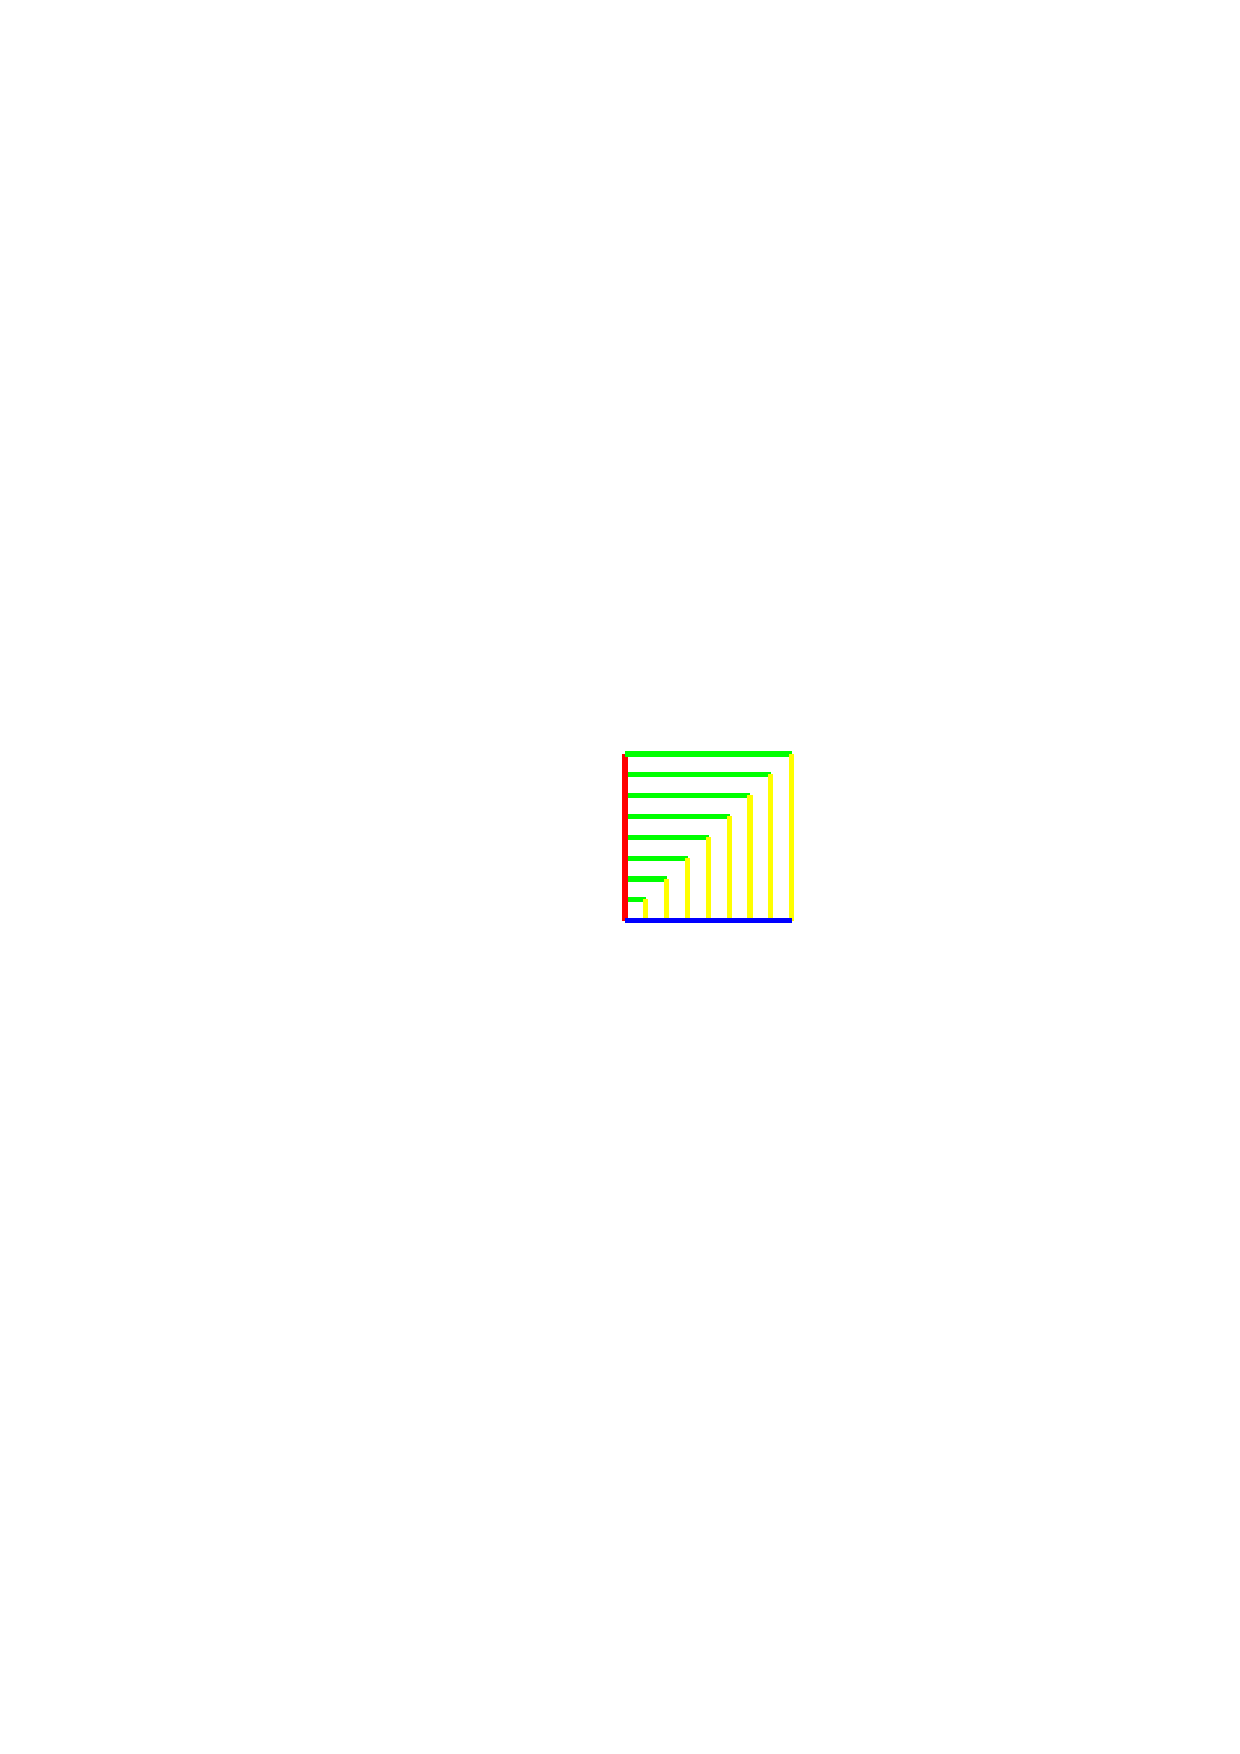
\includegraphics[clip,trim=10cm 11cm 6cm 11cm,scale=1.25]{../Pictures/out_tunnel.pdf}
\end{center}

\noindent Variables can be set using a postfix notation, e.g.~:
\begin{codesnippet}
START
   SET A ( 0 )
   SET B ( $A 1 + )
   SET C ( $B 2 * )
END
\end{codesnippet}

\subsection*{The Formal Grammar}
{\samepage
\begin{verbatim}
<PROG>   ::= "START" <INSLST>

<INSLST> ::= "END" | <INS> <INSLST>
<INS>    ::= <FWD> | <RGT> | <COL> | <LOOP> | <SET>

<FWD>    ::= "FORWARD" <VARNUM>
<RGT>    ::= "RIGHT" <VARNUM>
<COL>    ::= "COLOUR" <VAR> | "COLOUR" <WORD>
<LOOP>   ::= "LOOP" <LTR> "OVER" <LST> <INSLST>
<SET>    ::= "SET" <LTR> "(" <PFIX>

<VARNUM> ::= <VAR> | <NUM>
% Variables e.g. $A, $B, $Z etc.
<VAR>    ::= $<LTR>
% One Uppercase letter
<LTR>    ::= A, B ... Z
% Any valid double (as defined by scanf("%lf"...)
<NUM>    ::= 10 or -17.99 etc.

% A single word (as defined by scanf("%s"...) with double-quotes around it
% Valid colours include "BLACK", "RED", "GREEN", "BLUE",
% "YELLOW", "CYAN", "MAGENTA", "WHITE"
<WORD>   ::=  "RED", "BLUE", "HELLO!" or  "178"

<LST>    ::= "{" <ITEMS>
<ITEMS>  ::= "}" | <ITEM> <ITEMS>
<ITEM>   ::= <VARNUM> | <WORD>

<PFIX>   ::= ")" | <OP> <PFIX> | <VARNUM> <PFIX>
% A single mathematical operation character
<OP>     ::= + - / *
\end{verbatim}
}

\begin{exercise}

\strut\\[1em]
\vspace*{1ex}
\noindent{\bf\large Parser (35\%)}

\noindent Implement a recursive descent parser - this will report
whether or not a given turtle program follows the formal grammar or not.
The input file is specified via \verb^argv[1]^ - there is {\bf no}
output if the input file is {\bf valid}. Elsewise, a graceful non-zero
\verb^exit^ is made.  You should use the techniques described in the
lecture for this - writing code that carefully follows the grammar. For
instance, it won't use a tokenzier.

\noindent All source code will be in the \verb^Parse/^ sub-directory.

\vspace*{1em}
\noindent {\bf\large Interpreter (25\%)}

\noindent Extend the parser, so it becomes an interpreter. The
instructions are now `executed'. Do not begin a new program for this,
simply copy and then extend your existing parser. Output is to a text
file if the users specifies an \verb^argv[2]^, in the form of a 2D array
of characters where colours are represented by blac(K), (R)ed, (G)reen,
(Y)ellow, (B)lue, (M)agenta, (C)yan and (W)hite, via a $51$ wide $\times$
$33$ height array of characters e.g.:

\begin{verbatim}





                         GGGGGY
                         R    Y
                         R    Y
                         R    Y
                         R    Y
                      WWWWWWWWWWWW
                       W        W
                       W        W
                        W      W
                        W      W
                         W    W
                         W   W
                          W  W
                          W W
                           WW
                           W





\end{verbatim}

\noindent If no \verb^argv[2]^ is specified, then output is to the
screen using ANSI colour characters in same style as that used in
Section~\ref{sec:ansi}, with a $1$ second pause after each \verb^FORWARD^
instruction. 

\noindent Note that some files that successfully parse will not
successfully interpret (and vice versa) - there are example \verb^.ttl^
files provided to demonstrate this.

\noindent All interpreter source code will be in the \verb^Interp/^ sub-directory.

\vspace*{1em}
\noindent {\bf\large Postscript (5\%)}

\noindent Extend the output functionality of the
interpreter such that if \verb^argv[2]^ has a \verb^.ps^
extension, then the correct postscript instructions are written to that file.
\wwwurl{https://paulbourke.net/dataformats/postscript} Since PDFs are a
more common file format, then at the end, your program should also convert the \verb^.ps^
file to a \verb^.pdf^ file using a \verb^system()^ call in your C code
to \verb^ps2pdf^ which is installed on the lab machines. 
My implementation uses the postscript commands \verb^showpage^,
\verb^newpath^, \verb^moveto^, \verb^lineto^, \verb^setrgbcolour^, \verb^scale^
and \verb^stroke^.

If you get this to work, add it to the interpreter above - it will be tested
using both \verb^.txt^ and \verb^.ps^ output modes.

\vspace*{1ex}
\noindent {\bf\large Extension (15\%)}

\noindent Extend the project in a direction of
your choice. It should demonstrate your {\bf understanding} of some aspect
of programming or S/W engineering. If you extend the formal grammar
make sure that you give us the new, full grammar, along with the code in
the \verb^Extension/^ sub-directory named \verb^grammar.txt^, in addition to
a $300$ word (max) description of what you've achieve in \verb^extension.txt^.
Please do not submit ideas for future work, only functionality you've got working.

\vspace*{1ex}
\noindent {\bf\large Testing (20\%)}

\noindent Show the testing strategy on your code -
you should give details of any
unit testing or white/black-box testing done on your code. Describe any
test-harnesses used. Convince us that every line of your C code has
been tested, explaining the process, lessons learned and bugs found.
Submit a file \verb^testing.txt^ in the sub-directory \verb^Testing/^.

\subsection*{Hints}
\begin{itemize}

\item Understand the noughts and ones example given in the notes.

\item Don't try to write the entire program in one go. Try a cut
down version of the grammar first, e.g.:
{\small
\begin{verbatim}
<PROG>   ::= "START" <INSLST>

<INSLST> ::= "END" | <INS> <INSLST>
<INS>    ::= <FWD> | <RGT>

<FWD>    ::= "FORWARD" <NUM>
<RGT>    ::= "RIGHT" <NUM>

<NUM>    ::= 10 or -17.99 etc.
\end{verbatim}
}

\item The language is simply a sequence of words (even the braces),
so use \verb^fscanf()^.

\item Some issues, (e.g. drawing out-of-bounds), incorrect postfix
expressions cannot explained by the formal grammar. Use your own
common-sense to decide how to reconcile these, and explain what you
have done.

\item Once your parser works, extend it to become an interpreter. DO
NOT aim to parse the program first and then interpret it
separately. Interpreting and parsing are inseparably bound together. Use
our lectures notes for this and not those from other units such as
Architecture which take a very slightly different approach.

\item For the simple trigonometry required to compute the turtles
destination, bear in mind that the \verb^cos()^ and \verb^sin()^ functions
in C require parameters in radians and not degrees.

\item The turtle always begins in the centre of the screen facing due
north (upwards) and having a default white colour.  For the postscript/PDF
part, since white ink is hard to see on white paper, I've redefined
white ink to be slightly grey.

\item Start testing very early - this is a complex program to test and
trying to do it (or explain it) near the end won't work.

\end{itemize}

\subsection*{Submission}
Adapt the given Makefile if necessary to allow the parser, interpreter and extension to 
be built.
Submit your extension via text files \verb^extension.txt^ in \verb^Extension/^ along with  \verb^grammar.txt^ and your source code.

Your testing strategy will be explained in \verb^testing.txt^ along with any other files you'd like to bring our attention to in \verb^Testing/^.

Bundle this all up into a single \verb^turtle.zip file^ that contains {\bf everything} required
for us to compile and understand your code.

\end{exercise}

